\documentclass[11pt]{article}
\usepackage[a4paper,margin=1in]{geometry}
\usepackage{amsmath}
\usepackage{amssymb}
\usepackage{booktabs}
\usepackage{graphicx}
\usepackage{hyperref}
\graphicspath{{figures/}}

\title{Constraint-Integrated Hierarchical Score-to-Score Transformer for Explainable SATB Harmonization}
\author{Author information omitted for review}
\date{}

\begin{document}
\maketitle

\begin{abstract}
Four-part SATB harmonization is not fully characterized by token likelihood. A generated score may match local pitch distributions while violating voice ranges, vertical spacing, parallel-motion constraints, seventh resolution, or cadence conventions that define common-practice chorale writing. This manuscript reformulates SATB harmonization as a score-level neural-symbolic generation problem in which a hierarchical Transformer proposes symbolic pitch sequences and a rule-aware decoding objective penalizes musically localized violations. The proposed Constraint-Integrated Hierarchical Score-to-Score Transformer (CIH-S2S Transformer) combines harmonic-plan conditioning, explicit same-timestep voice-relation modeling, bar-level temporal context, iterative masked refinement, MusicXML export, and localized rule reporting. The artifact-backed evaluation uses 371 music21 Bach chorales encoded on a 0.25-quarter-note grid with a deterministic 297/37/37 train/validation/test split and SATB voice order. In three-seed same-split experiments, the vanilla Transformer reports pitch-token accuracy 0.7691, cross entropy 0.8705, and 15.3312 automatic rule flags per 100 score positions. The current rule-guided Transformer reports 0.8230, 0.6073, and 3.6549, respectively. CIH-S2S reports the best likelihood-oriented metrics among these three Transformer families, with pitch-token accuracy 0.8306 and cross entropy 0.5658, but its total automatic rule flags remain 14.4702 per 100 positions. A full-test decoder analysis on one trained CIH-S2S checkpoint shows that constrained beam search reduces parallel-fifth and parallel-octave diagnostics relative to neural argmax, while not uniformly reducing total automatic rule flags. These findings support the usefulness of explicit rule diagnostics and constraint-aware decoding in this same-corpus setting. They do not establish state-of-the-art performance, expert preference, complete symbolic constraint solving, or external-corpus robustness; expert evaluation and a curated external benchmark remain pending.
\end{abstract}

\section{Introduction}

Automatic SATB harmonization asks a model to complete or generate four coordinated vocal lines, typically soprano, alto, tenor, and bass, under tonal, contrapuntal, and notational constraints. In this setting, the target is not only a sequence of likely pitch tokens. A harmonization must also form plausible vertical sonorities, keep each voice in a singable range, avoid inappropriate crossing and spacing, manage parallel fifths and octaves, resolve tendency tones, and articulate cadences. Token likelihood and voice-leading correctness are therefore related but non-identical objectives.

This distinction matters for neural sequence models. A model trained only to maximize conditional likelihood can learn frequent local pitch events while still producing errors that are sparse in the token stream but musically salient. A few unresolved sevenths or parallel octaves can dominate the perceived quality of an otherwise plausible chorale texture. Conversely, a purely symbolic rule system can reduce certain violations but may lack flexibility, stylistic adaptation, and support for partially observed score completion. SATB harmonization is thus a useful test case for neural-symbolic score generation: the model must combine distributional learning with interpretable musical constraints.

We study explainable score-level SATB harmonization with MusicXML output. The input may be a soprano melody, a bass line, or a partially masked SATB score. The output is a four-voice symbolic score and a localized report of common-practice harmony and counterpoint diagnostics. The main research question is whether explicit harmonic conditioning, same-timestep voice interaction, iterative refinement, and constraint-aware decoding can make a neural harmonizer more transparent and more compatible with voice-leading evaluation than a vanilla Transformer baseline.

The paper makes five contributions. First, it defines a hierarchical score-level SATB modeling framework in which harmonic context, bass planning, inner-voice decoding, and final refinement are separated rather than flattened into independent token streams. Second, it incorporates harmonic-plan conditioning with key, beat, measure, phrase-end, chord-root, chord-quality, Roman-numeral, dominant-function, and seventh-chord features, while preserving a dedicated unknown embedding for unavailable labels. Third, it formulates neural-symbolic constrained decoding as a bounded search problem combining neural proposal probabilities with hard and soft voice-leading constraints. Fourth, it connects generation to MusicXML export and localized rule reports, allowing each generated score to be inspected as a musical artifact rather than only as a token array. Fifth, it provides a reproducible evaluation protocol with deterministic splits, source-data-backed figures, multi-seed summaries where available, and explicit claim boundaries for pending expert and external-source evaluations.

The empirical results in this revision are intentionally conservative. The repository contains formal same-corpus three-seed results for the vanilla Transformer, current rule-guided Transformer, and CIH-S2S Transformer, a single-seed LSTM row, selected single-run ablations, and a one-checkpoint full-test constraint-decoder analysis. Accordingly, the Results section reports only values that are traceable to recorded CSV, JSON, checkpoint, figure-source, or evaluation artifacts.

\section{Related Work}

Computational chorale harmonization has long served as a benchmark for modeling tonal structure. Early neural work such as HARMONET showed that learned systems could approximate Bach-style chorale harmonization under constrained representations \cite{hild1992harmonet}. Later deep generative models, including DeepBach, modeled chorales with conditional neural architectures and pseudo-Gibbs sampling, enabling steerable generation from partially observed scores \cite{hadjeres2017deepbach}. Coconet framed counterpoint as an orderless infilling problem, demonstrating the value of masked score completion for polyphonic music \cite{huang2017coconet}. Broader surveys describe the diversity of symbolic music generation settings, including sequence models, piano-roll models, and rule-aware systems \cite{briot2020deep}.

SATB harmonization differs from generic symbolic sequence generation because the voices form a coordinated notated texture. The soprano, alto, tenor, and bass lines are not independent streams; they define vertical intervals at each timestep and temporal motion across adjacent timesteps. This creates a gap between language-model-style next-token prediction and common-practice voice-leading evaluation. A pitch token can be locally probable while participating in a voice crossing, a spacing violation, a parallel octave, or an unresolved chordal seventh.

The present work uses music21 for score parsing and symbolic-music processing \cite{cuthbert2010music21}. Its contribution is not a claim that a Transformer alone solves chorale harmonization. Instead, the system treats a neural model as a proposal mechanism and exposes rule diagnostics during decoding and evaluation. This places the work between neural chorale generation and interpretable symbolic checking: the neural model learns score distributions, while the symbolic layer supplies musically named constraints and localized reports.

\section{Task and Score Representation}

Let $X$ denote the observed score context and $Y$ denote the missing or generated SATB tokens. The system supports two primary tasks. In soprano-to-SATB harmonization, the soprano line is observed and the alto, tenor, and bass voices are predicted. In masked SATB infilling, a subset of tokens in an existing four-voice score is masked and the model predicts the missing entries. The same representation can also support bass-to-SATB and partial-score completion, but the formal results reported here focus on soprano-to-SATB and masked infilling.

The main dataset is the music21 Bach chorale collection. The current processed artifact contains 371 encoded chorales, split deterministically into 297 training, 37 validation, and 37 test scores. Scores are quantized on a 0.25-quarter-note grid and truncated or padded to sequence length 256. The token tensor has shape $371 \times 256 \times 4$, with voice order soprano, alto, tenor, bass. The vocabulary contains 53 symbolic pitch tokens, including special tokens for padding and masking.

Each training item contains the full token matrix, an input matrix in which prediction targets are replaced by a mask token, a known-position mask, a target mask, and a valid-position mask. The training loss is computed over target positions and ignores padding. Harmonic metadata are represented at the timestep level: key tonic pitch class, beat position, measure index, phrase-end flag, chord root, chord quality, Roman numeral, dominant-function flag, seventh-chord flag, and known-label indicators. Unavailable harmonic labels are not imputed. They are represented by a dedicated \texttt{UNKNOWN} identifier, preserving the distinction between unknown labels and known harmonic categories.

\section{Proposed Method}

\subsection{Overview}

The proposed CIH-S2S Transformer is designed as a score-to-score architecture for four-voice symbolic music. It separates three sources of structure: horizontal temporal context within each voice, vertical sonority across voices at the same timestep, and harmonic-plan information over beats and measures. The model returns logits in the same shape as the existing evaluation and MusicXML export pipeline, $B \times T \times 4 \times V$, where $B$ is batch size, $T$ is sequence length, four indexes SATB voices, and $V$ is vocabulary size.

\begin{figure}[t]
\centering
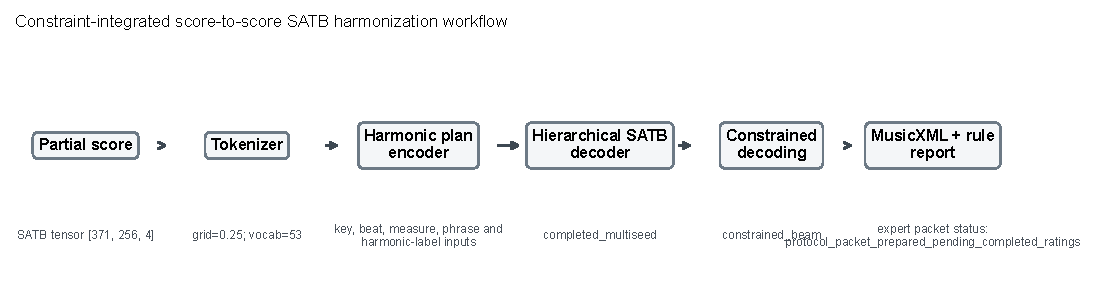
\includegraphics[width=\linewidth]{figure1_system_structure.pdf}
\caption{System structure for score-level neural-symbolic SATB harmonization. Partial score context is tokenized with harmonic metadata, encoded by the harmonic-plan encoder, decoded by the hierarchical SATB decoder, filtered by bounded constraint-aware decoding, and exported as MusicXML with localized rule reports. The figure is generated from \texttt{paper/figures/source\_data/figure1\_system\_structure\_source.csv} and is a system schematic, not performance evidence.}
\label{fig:method}
\end{figure}

\subsection{Harmonic Plan Encoder}

The harmonic plan encoder embeds both observed score tokens and symbolic harmonic features. Token embeddings are combined with voice embeddings and known-position embeddings, allowing the model to distinguish observed soprano or bass material from masked targets. Harmonic inputs include key, beat, measure, phrase-end flag, chord root, chord quality, Roman numeral, dominant-function flag, seventh-chord flag, and known-label flags. Chord quality and Roman numeral IDs reserve index zero for unknown labels. This is important because automatically extracted harmonic annotations can be incomplete or ambiguous; the model should not convert missing labels into fabricated harmonic evidence.

The encoder produces timestep-level contextual states and lightweight bar-level summaries. Bar summaries pool local timestep states by measure index and project them back to the timestep sequence. This gives the decoder access to phrase-scale harmonic context without requiring memory-intensive global attention over long score sequences.

\subsection{Hierarchical SATB Decoder}

The decoder is hierarchical in the sense that it does not treat the four voices as a single undifferentiated flattened stream. A bass-skeleton head first estimates the bass distribution from the encoded context and harmonic plan. The resulting bass representation is then fed into inner-voice decoding for alto and tenor, followed by final voice-specific pitch projections. This staged design reflects the role of the bass in tonal harmony while keeping the output compatible with the existing tensor interface.

The hierarchy should be understood as architectural conditioning, not as additional supervised labels. The current training objective remains masked pitch-token cross entropy over the target positions:
\[
\mathcal{L}_{\mathrm{CE}}(\theta) =
- \sum_{t,v} m_{t,v}\log p_{\theta}(y_{t,v}\mid X,H),
\]
where $m_{t,v}$ is the target mask for timestep $t$ and voice $v$, and $H$ denotes harmonic metadata.

\subsection{Voice-Relation Attention}

SATB voice leading depends on vertical relationships at the same timestep. The model therefore includes a voice-relation attention block that mixes the four voice states within each timestep before final pitch prediction. This block explicitly models vertical sonority and voice spacing rather than requiring the temporal Transformer alone to infer them from flattened tokens. The module can be ablated with the configuration flag \texttt{use\_voice\_relation\_attention: false}.

\subsection{Temporal and Bar-Level Attention}

The temporal path uses relative or local score context to model melodic continuity and short-range contrapuntal motion. The bar-summary path provides a lower-memory route for measure-level information. This is intended for RTX 4060-class hardware: the model avoids very large attention windows and provides smaller 8GB and 16GB configurations.

\subsection{Iterative Masked Refinement}

Generation can be refined over multiple passes. After an initial prediction, low-confidence target positions may be remasked and decoded again while preserving higher-confidence predictions. This procedure allows each pass to update local vertical and temporal context. The refinement count is configurable, and the no-refinement ablation disables this step.

\section{Constraint-Aware Decoding}

The decoding objective combines neural likelihood with symbolic rule costs:
\[
\hat{Y} =
\arg\max_{Y \in \mathcal{Y}}
\left[
\log p_\theta(Y\mid X,H) - \sum_i \lambda_i R_i(Y)
\right]
\quad \text{subject to } C_j(Y)=1,\; j=1,\ldots,J .
\]
Here $R_i(Y)$ are soft rule costs, $\lambda_i$ are non-negative weights, and $C_j(Y)$ are hard constraints. In the implemented bounded beam-search decoder, the neural model proposes top-$k$ pitch candidates. Candidate beams are expanded, hard-constraint violations are filtered when valid alternatives exist, and the remaining candidates are scored by neural log probability minus weighted rule cost.

The hard constraints include SATB voice range, voice crossing, adjacent-voice spacing, parallel fifths, parallel octaves, unresolved chordal seventh diagnostics, leading-tone resolution diagnostics, and final-cadence legality checks. The soft costs include melodic smoothness, common-tone retention, contrary-motion preference, cadence strength, stylistic-similarity proxy, and singability proxy. These labels describe automatic diagnostics and decoding preferences. They should not be interpreted as complete music-theoretic proof of correctness.

The current decoder is a pure Python constrained beam-search backend. It is not a CP-SAT or ILP solver, and it is not guaranteed to find the global optimum of the constrained problem. This distinction is important for the claim boundary: the system implements bounded constraint-aware decoding, not complete formal constraint solving.

\section{Experimental Setup}

\subsection{Dataset and Split}

The primary dataset is the music21 Bach chorale collection, encoded as 371 SATB scores. The deterministic split contains 297 training chorales, 37 validation chorales, and 37 held-out test chorales. The sequence length is 256, the quantization grid is 0.25 quarter length, and the voice order is soprano, alto, tenor, bass. The main soprano-to-SATB task keeps the soprano voice observed and predicts alto, tenor, and bass. The masked-infilling task uses Bernoulli masking over SATB tokens according to the task configuration.

\subsection{Baselines and Model Variants}

The current evidence package includes the following same-split baselines and variants: an LSTM baseline, a vanilla Transformer without rule-guided constraints, the current rule-guided Transformer, the CIH-S2S Transformer, a masked-infilling variant, and component ablations. Vanilla Transformer, current rule-guided Transformer, and CIH-S2S rows have three formal seeds on the deterministic Bach split. The LSTM and component ablations are single-run rows and are interpreted as narrower evidence.

DeepBach-style pseudo-Gibbs and Coconet-style infilling baselines are relevant comparators for the final article, but repository artifacts currently mark them as TODO rather than completed results. They are discussed as planned baselines, not as evaluated rows.

\subsection{External-Source Protocol}

BCFB and CPDL source-chain experiments are treated as external-source pilots. The BCFB subset is Bach-related material and is not a true external repertory benchmark. The CPDL subset is an automatically selected MusicXML candidate set and still requires license filtering, SATB candidate curation, and a documented split before it can support claims about external generalization. The present manuscript therefore does not claim external-corpus robustness.

\subsection{Expert Evaluation Protocol}

The expert evaluation protocol uses anonymized score packets containing ground truth, vanilla Transformer outputs, current rule-guided Transformer outputs, and CIH-S2S outputs. The planned dimensions cover harmonic correctness, voice leading, seventh resolution, cadence quality, singability, stylistic consistency, pedagogical usefulness, and overall preference. At the time of this revision, no returned expert ratings are available. Expert evaluation is therefore pending and no human-preference result is reported.

\section{Evaluation Metrics}

The evaluation reports pitch-token accuracy, voice-wise accuracy, cross entropy, and negative log likelihood over held-out target tokens. Automatic rule diagnostics are normalized per 100 score positions and include total rule flags, parallel fifths, parallel octaves, voice crossing, adjacent-voice spacing, range violation, seventh-resolution diagnostics, leading-tone diagnostics, cadence unknown rate, and cadence correctness when cadence labels are detected. Harmonic coverage metrics report Roman-numeral extraction coverage, chord-label coverage, generated-score Roman-numeral coverage, and generated-score chord-label coverage. Generation validity is tracked through MusicXML export success and evaluated generation count.

Statistical reporting is conservative. Mean and standard deviation are reported only where repeated formal seeds exist. For the three Transformer families, seeds 2026, 2027, and 2028 are shared, so paired seed-level summaries are available. Because $n=3$ is small and SciPy is not required by the local environment, the statistical summary uses an exact Wilcoxon signed-rank fallback. The resulting $p$ values are reported as exploratory checks rather than as strong evidence of significance.

\section{Results}

\subsection{Held-Out Bach Test Split}

Table~\ref{tab:main-results} summarizes the formal same-split rows used in the main comparison. Vanilla Transformer, current rule-guided Transformer, and CIH-S2S values are means over seeds 2026, 2027, and 2028. The LSTM row is a single recorded baseline. The current rule-guided Transformer improves pitch-token accuracy and cross entropy relative to the vanilla Transformer while substantially reducing automatic rule flags. CIH-S2S records the highest pitch accuracy and lowest cross entropy among the three Transformer families, but it does not reduce total automatic rule flags to the level of the current rule-guided decoder.

\begin{table}[t]
\centering
\caption{Held-out Bach test results for recorded same-split models. Values are read from \texttt{results/project1\_metrics.csv}, \texttt{results/project1\_robustness\_summary.json}, \texttt{results/vanilla\_transformer\_robustness\_summary.json}, and \texttt{results/cih\_s2s\_robustness\_summary.json}. Rule flags are automatic diagnostics per 100 score positions. LSTM is single-seed; the Transformer-family rows are three-seed means.}
\label{tab:main-results}
\begin{tabular}{lrrrr}
\toprule
Model & Accuracy & CE & Rule flags & XML \\
\midrule
LSTM baseline & 0.7771 & 0.7810 & 12.9151 & 1.0000 \\
Vanilla Transformer & 0.7691 & 0.8705 & 15.3312 & 1.0000 \\
Current rule-guided Transformer & 0.8230 & 0.6073 & 3.6549 & 1.0000 \\
CIH-S2S Transformer & 0.8306 & 0.5658 & 14.4702 & 1.0000 \\
\bottomrule
\end{tabular}
\end{table}

\begin{figure}[t]
\centering
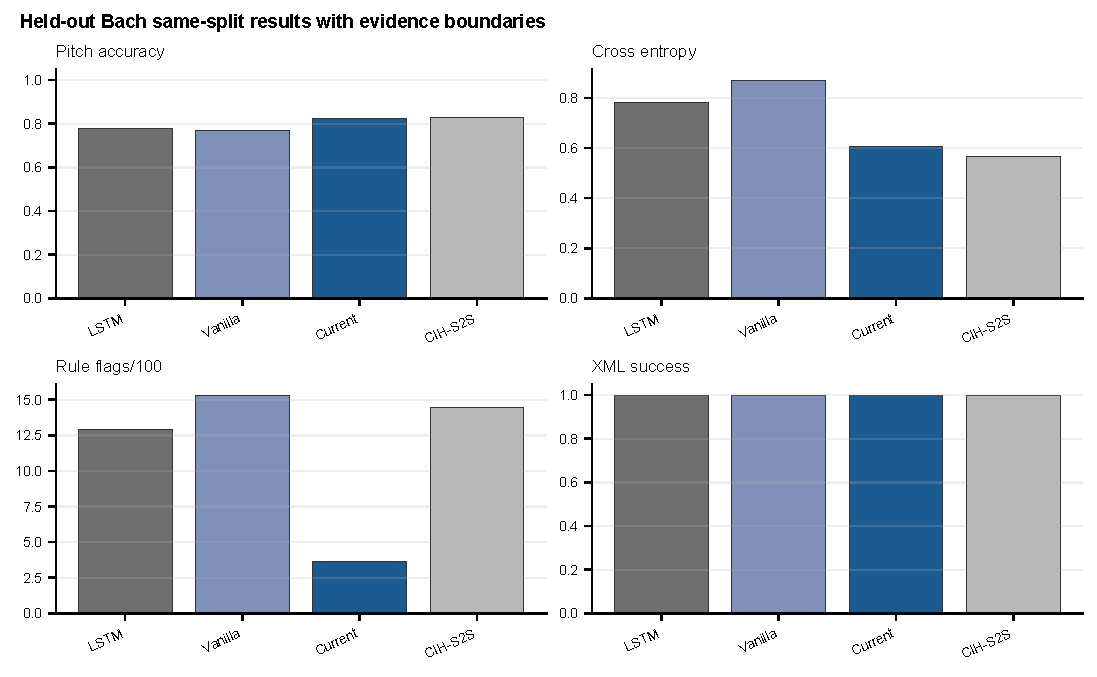
\includegraphics[width=\linewidth]{figure2_main_results.pdf}
\caption{Pitch-token accuracy, cross entropy, automatic rule flags, and MusicXML export success for the recorded Bach test split. The figure is generated from \texttt{paper/figures/source\_data/figure2\_main\_results\_source.csv}. Transformer-family rows are three-seed means when formal robustness summaries are available. The figure reports automatic metrics only and does not imply state-of-the-art performance or expert preference.}
\label{fig:metrics}
\end{figure}

The plotted rule diagnostics in Figure~\ref{fig:rules} show a sharper distinction than token accuracy alone. In the three-seed robustness summaries, the vanilla Transformer records 2.7631 parallel-fifth and 2.3326 parallel-octave flags per 100 positions, while the current rule-guided row records 0.0088 and 0.0439 respectively. The same row reports total automatic rule flags of 3.6549 per 100 positions. These are automatic checks over generated symbolic scores; they do not by themselves prove human musical preference.

\begin{figure}[t]
\centering
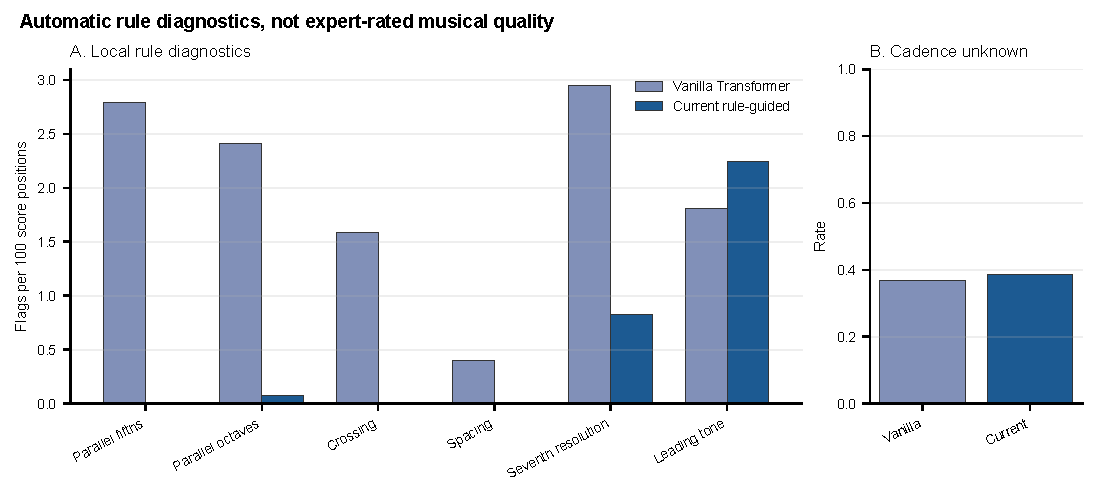
\includegraphics[width=\linewidth]{figure3_rule_diagnostics.pdf}
\caption{Automatic rule-diagnostic comparison for the held-out Bach test split. Source data are stored in \texttt{paper/figures/source\_data/figure3\_rule\_diagnostics\_source.csv}. The diagnostics identify localized rule flags, not expert-rated musical quality, and no confidence interval or significance test is included in this figure.}
\label{fig:rules}
\end{figure}

\subsection{Multi-Seed Robustness}

Three formal seeds are available for the vanilla Transformer, current rule-guided Transformer, and CIH-S2S Transformer: 2026, 2027, and 2028. The repeated-seed summary in Table~\ref{tab:multiseed} reports mean and standard deviation over those seeds. CIH-S2S has the highest mean pitch accuracy and lowest mean cross entropy in this matched comparison. The current rule-guided Transformer has the lowest total automatic rule-flag rate.

\begin{table}[t]
\centering
\caption{Three-seed descriptive summary for the matched Transformer-family comparison. Values are read from formal robustness summaries under \texttt{results/}. Rule flags are automatic diagnostics per 100 score positions.}
\label{tab:multiseed}
\begin{tabular}{lrrr}
\toprule
Model & Accuracy & CE & Rule flags \\
\midrule
Vanilla Transformer & 0.7691 $\pm$ 0.0015 & 0.8705 $\pm$ 0.0019 & 15.3312 $\pm$ 1.3316 \\
Current rule-guided Transformer & 0.8230 $\pm$ 0.0013 & 0.6073 $\pm$ 0.0117 & 3.6549 $\pm$ 0.1196 \\
CIH-S2S Transformer & 0.8306 $\pm$ 0.0031 & 0.5658 $\pm$ 0.0174 & 14.4702 $\pm$ 1.6440 \\
\bottomrule
\end{tabular}
\end{table}

\begin{figure}[t]
\centering
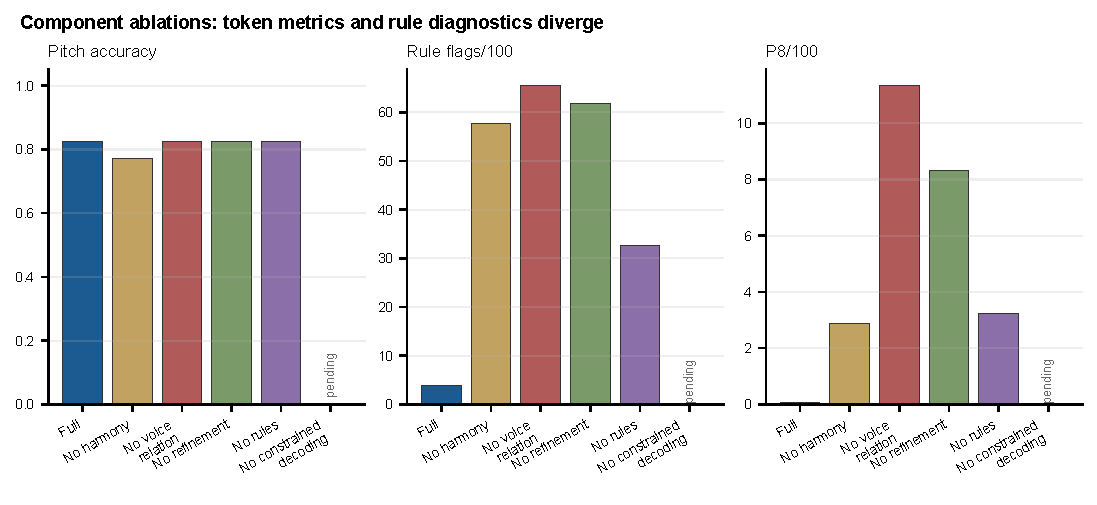
\includegraphics[width=\linewidth]{figure4_ablation.pdf}
\caption{Component ablations for the recorded Bach soprano-to-SATB task. Source data are stored in \texttt{paper/figures/source\_data/figure4\_ablation\_source.csv}. Rows are single-run automatic evaluations unless otherwise stated; the figure should therefore be read as component evidence rather than a multi-seed significance result.}
\label{fig:ablation}
\end{figure}

Paired seed-level comparisons are available for these three Transformer-family rows. The exact Wilcoxon fallback reports $p=0.25$ for CIH-S2S versus vanilla pitch accuracy and cross entropy, $p=0.50$ for CIH-S2S versus vanilla total rule flags, and $p=0.25$ for CIH-S2S versus current rule-guided pitch accuracy, cross entropy, and total rule flags. These small-sample tests are useful as traceable statistical summaries, but they are not strong significance evidence.

\subsection{Ablation Evidence}

The component ablations in Table~\ref{tab:ablations} indicate that accuracy alone can miss musically important failure modes. Removing harmonic conditioning reduces pitch-token accuracy to 0.7716 and increases cross entropy to 0.8469. Removing iterative refinement leaves token accuracy similar but raises automatic rule flags to 61.7290 per 100 positions and parallel-octave flags to 8.3158. Removing rule-guided decoding leaves accuracy similar but raises automatic rule flags to 32.6173. Removing voice-relation attention again leaves token accuracy similar but raises automatic rule flags to 65.4718 and parallel-octave flags to 11.3337. These ablations support the central methodological point: token accuracy is not a sufficient proxy for voice-leading behavior.

\begin{table}[t]
\centering
\caption{Recorded component ablations for the Bach soprano-to-SATB task. Values are single-run automatic evaluations from \texttt{results/project1\_metrics.csv}. No significance test is included.}
\label{tab:ablations}
\begin{tabular}{lrrrr}
\toprule
Variant & Accuracy & CE & Rule flags & P8 \\
\midrule
Full rule-guided row & 0.8233 & 0.5942 & 3.7823 & 0.0791 \\
No harmonic conditioning & 0.7716 & 0.8469 & 57.7491 & 2.8861 \\
No iterative refinement & 0.8249 & 0.5938 & 61.7290 & 8.3158 \\
No rule-guided decoding & 0.8238 & 0.5936 & 32.6173 & 3.2156 \\
No voice-relation attention & 0.8246 & 0.5863 & 65.4718 & 11.3337 \\
\bottomrule
\end{tabular}
\end{table}

\subsection{Masked Infilling and MusicXML Export}

The masked-infilling variant records pitch-token accuracy of 0.8290 and cross entropy of 0.5866 on the same held-out split, with MusicXML export success of 1.0000 over 37 evaluated generations. This supports the claim that the same score representation and export pathway can handle both soprano-to-SATB and masked SATB infilling. It does not imply that all input-score conditions have been exhaustively evaluated.

\subsection{CIH-S2S Constraint-Decoder Analysis}

Figure~\ref{fig:constraint-decoder} reports a full-test decoder analysis for one trained CIH-S2S checkpoint. Neural argmax records 11.8055 total automatic rule flags per 100 positions, with 1.5034 parallel fifths and 3.2804 parallel octaves per 100 positions. Local rule repair lowers total flags to 11.2488 but leaves the same P5 and P8 rates. Constrained beam search changes the trade-off: the largest beam setting tested, $b=8,k=12$, lowers P5/P8 to 0.1430/0.3041 per 100 positions, but total automatic rule flags remain 13.0082 per 100 positions and runtime rises to 27.6892 seconds per score. This result supports the need for multi-objective decoder analysis rather than a single ``rule reduction'' claim.

\begin{figure}[t]
\centering
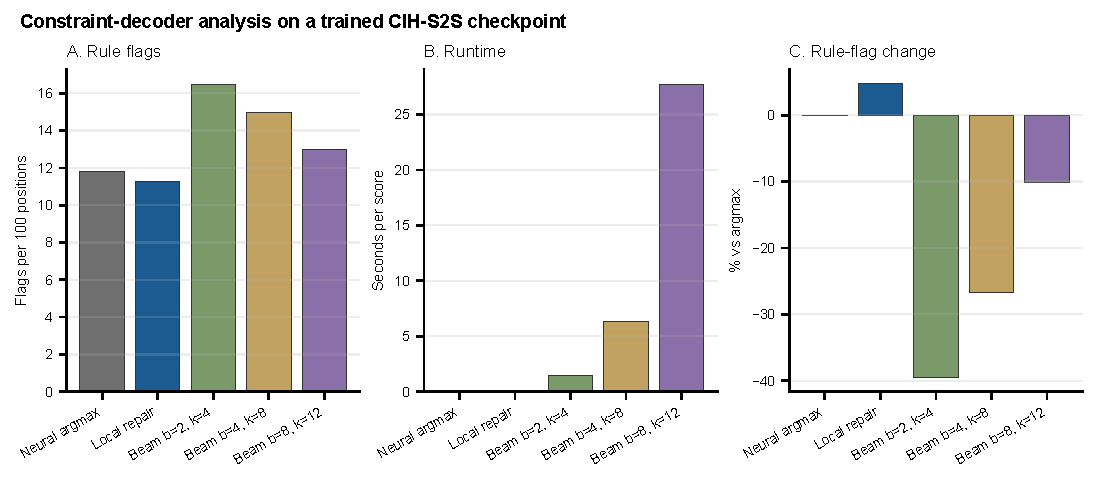
\includegraphics[width=\linewidth]{figure5_constraint_decoder_analysis.pdf}
\caption{Constraint-decoder analysis on the full Bach test split for one formally trained CIH-S2S checkpoint. Source data are stored in \texttt{results/constraint\_decoder\_analysis\_summary.csv} and \texttt{results/constraint\_decoder\_analysis.csv}. Negative rule-flag change values indicate more total automatic flags than neural argmax. No expert rating, confidence interval, or significance test is included.}
\label{fig:constraint-decoder}
\end{figure}

\subsection{Training Curves and Expert-Evaluation Materials}

Figure~\ref{fig:training-curves} summarizes validation cross entropy and validation accuracy for runs with complete recorded logs. The curves are included to make optimization behavior inspectable, not to replace held-out test metrics or paired seed summaries.

\begin{figure}[t]
\centering
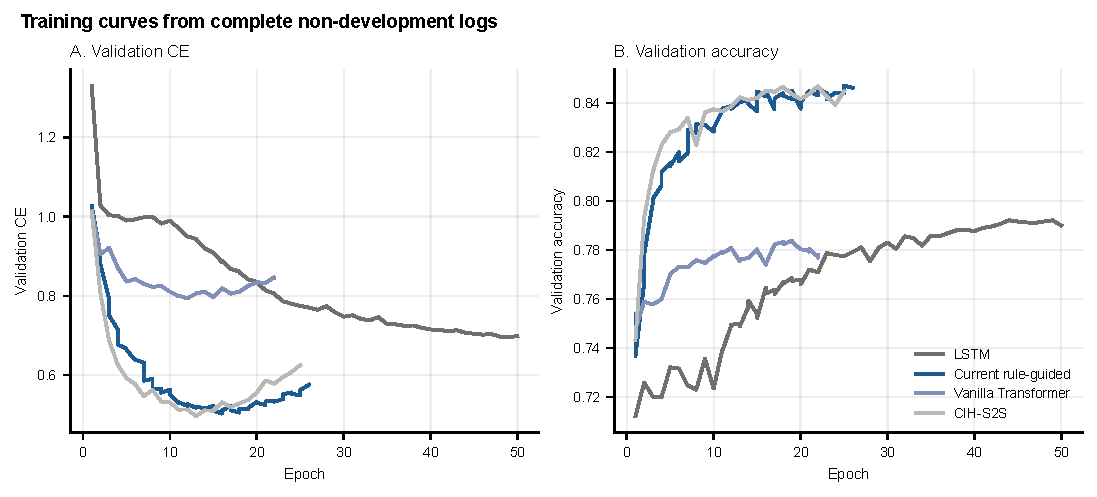
\includegraphics[width=\linewidth]{figure6_training_curves.pdf}
\caption{Training curves for runs with complete validation logs. Source data are stored in \texttt{paper/figures/source\_data/figure6\_training\_curves\_source.csv}; excluded or incomplete logs are listed in \texttt{paper/figures/source\_data/figure6\_training\_curve\_exclusions.csv}. The figure reports logged validation metrics only and does not include a significance test.}
\label{fig:training-curves}
\end{figure}

Figure~\ref{fig:expert-protocol} documents the prepared blind evaluation protocol. No completed expert ratings are available at the time of this revision, so the figure is a protocol artifact rather than a result panel.

\begin{figure}[t]
\centering
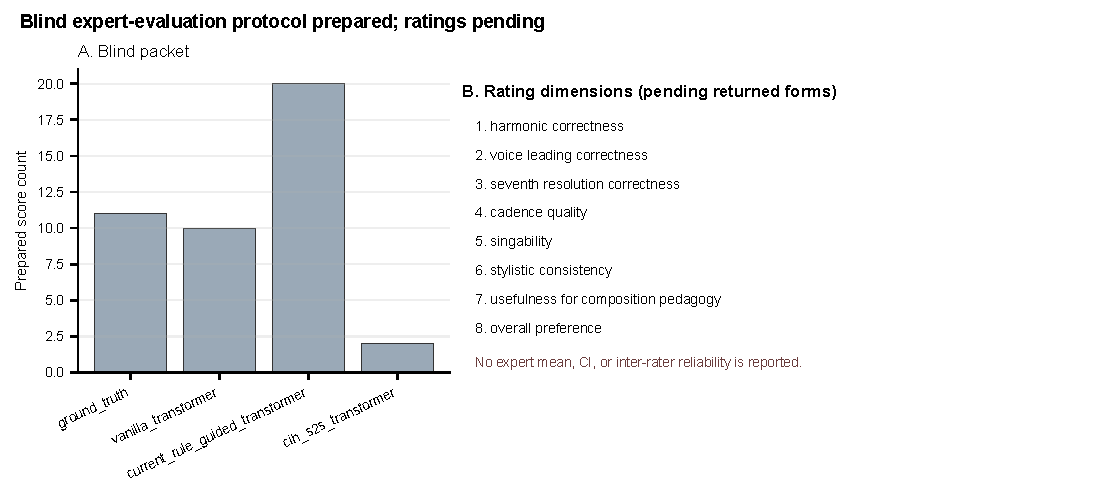
\includegraphics[width=\linewidth]{figure7_expert_protocol.pdf}
\caption{Prepared blind expert-evaluation protocol for ground-truth, vanilla Transformer, current rule-guided Transformer, and CIH-S2S outputs. Source data are stored in \texttt{paper/figures/source\_data/figure7\_expert\_protocol\_source.csv}. No returned ratings, confidence intervals, or inter-rater reliability estimates are available yet.}
\label{fig:expert-protocol}
\end{figure}

\section{Discussion}

The results illustrate three distinct notions of performance. The first is likelihood-based performance, measured by cross entropy and token accuracy. These metrics assess whether generated tokens match the held-out Bach tokens under the chosen representation and masking scheme. The second is rule-diagnostic performance, measured by automatic flags for parallel motion, spacing, crossing, seventh resolution, and related checks. These diagnostics inspect generated symbolic scores and identify localized voice-leading concerns. The third is human musicality, which includes style, phrase shape, singability, pedagogical usefulness, and listener or expert preference.

The distinction among these levels is central. The ablations show cases in which token accuracy stays near the full model while automatic rule flags increase sharply. This suggests that likelihood metrics alone can understate musically salient errors. At the same time, automatic rule diagnostics are not a substitute for expert evaluation. They encode selected common-practice checks and are sensitive to the reliability of harmonic labels, cadence detection, and symbolic parsing. A model with fewer rule flags can still produce unconvincing phrases, and a model with occasional flags may still contain musically acceptable idioms.

The practical value of the neural-symbolic approach is that it makes these levels inspectable. MusicXML export allows generated scores to be viewed in notation software, while localized rule reports allow developers, music theorists, and educators to identify where a generated score conflicts with selected voice-leading rules. This is more informative than a scalar token score alone and provides a basis for future expert evaluation.

The CIH-S2S results refine the interpretation of the proposed upgrade. Harmonic-plan conditioning, bar-level context, voice-relation attention, iterative refinement, and hierarchical decoding improve likelihood-oriented metrics relative to the vanilla Transformer and the current rule-guided Transformer in the same-corpus three-seed comparison. However, the automatic rule diagnostics reveal a trade-off: CIH-S2S does not inherit the low total rule-flag rate of the current local rule-guided decoder. The constraint-decoder analysis further shows that constrained beam search can reduce specific perfect-interval diagnostics while increasing or only partially reducing total rule flags. The appropriate claim is therefore not that CIH-S2S is globally superior, but that it separates likelihood improvement, voice-relation modeling, and explicit decoder trade-offs in a way that can be audited from score-level artifacts.

\section{Limitations}

\begin{enumerate}
\item The primary evidence is limited to the music21 Bach chorale collection and a deterministic 297/37/37 same-corpus split; it does not establish broad repertory generalization.
\item Automatic Roman-numeral, chord-label, and cadence annotations can be incomplete or incorrect, and unknown labels are explicitly represented rather than treated as true harmonic categories.
\item The BCFB and CPDL source-chain artifacts are pilots and do not yet constitute a curated, license-filtered, representative external benchmark.
\item Automatic rule metrics are localized diagnostics and are not equivalent to blind expert evaluation or human musicality judgments.
\item The current constrained decoder is a bounded beam-search procedure and is not a globally optimal or complete constraint solver.
\end{enumerate}

\section{Reproducibility}

The evaluation is designed to be traceable from data preparation to figures. The repository records the processed dataset, formal metric CSV files, automatic rule-diagnostic CSV files, repeated-seed summaries, figure source data, experiment matrix, and statistical-status table. The claim audit accompanying this revision lists the exact files used for each reported number. CIH-S2S model and decoder code are implemented in the model and constraint-decoding modules, with 16GB, 8GB, and small execution-check configurations provided under the configuration directory.

Hardware and software metadata recorded in figure source data indicate an NVIDIA GeForce RTX 4060 Ti 16GB, Intel i5-12400F, Windows 11, Python 3.11.9, and PyTorch 2.11.0+cu128 for the plotted primary rows. The 8GB configuration reduces batch size and uses gradient accumulation and checkpointing. Reproducing the final submission should include the exact commands for dataset construction, training, evaluation, MusicXML export, figure regeneration, and manuscript compilation.

\section{Conclusion}

This manuscript reframes SATB harmonization as an explainable neural-symbolic score generation problem rather than a pure token prediction task. The artifact-backed results show that the current rule-guided Transformer improves same-corpus pitch-token and cross-entropy metrics relative to a vanilla Transformer while reducing selected automatic voice-leading flags. CIH-S2S further improves likelihood-oriented metrics in the matched three-seed comparison, reaching mean pitch-token accuracy 0.8306 and cross entropy 0.5658, but it does not yet reduce total automatic rule flags below the current rule-guided decoder. The constraint-decoder analysis shows that bounded beam search can reduce specific P5/P8 diagnostics at increased runtime while leaving total rule-cost trade-offs unresolved. Final publication claims should remain limited to traceable score-level results and should add expert-evaluation and curated external-benchmark evidence only after those artifacts are complete.

\section*{Data Availability}

The processed split metadata, aggregated evaluation tables, figure source data, benchmark manifests, and example MusicXML outputs supporting the findings are available in the accompanying repository at \url{https://github.com/niuyupeng/yinyue3}. Source corpora remain subject to their original distribution and licensing terms. The exact release tag or commit should be used for final archival citation. No archival DOI is asserted in this repository snapshot.

\section*{Code Availability}

The model, score representation, constraint-decoding, evaluation, configuration, and figure-generation source code are available at \url{https://github.com/niuyupeng/yinyue3}. Author metadata, the final software license, and archival release information should be finalized before publication.

\bibliographystyle{plain}
\bibliography{references}

\end{document}
